\def\year{2020}\relax
%File: formatting-instruction.tex
\documentclass[letterpaper]{article} % DO NOT CHANGE THIS
\usepackage{aaai20}  % DO NOT CHANGE THIS
\usepackage{times}  % DO NOT CHANGE THIS
\usepackage{helvet} % DO NOT CHANGE THIS
\usepackage{courier}  % DO NOT CHANGE THIS
\usepackage[hyphens]{url}  % DO NOT CHANGE THIS
\usepackage{graphicx} % DO NOT CHANGE THIS
\usepackage{subcaption}
\urlstyle{rm} % DO NOT CHANGE THIS
\def\UrlFont{\rm}  % DO NOT CHANGE THIS
\usepackage{graphicx}  % DO NOT CHANGE THIS
\frenchspacing  % DO NOT CHANGE THIS
\setlength{\pdfpagewidth}{8.5in}  % DO NOT CHANGE THIS
\setlength{\pdfpageheight}{11in}  % DO NOT CHANGE THIS
%\nocopyright
%PDF Info Is REQUIRED.
% For /Author, add all authors within the parentheses, separated by commas. No accents or commands.
% For /Title, add Title in Mixed Case. No accents or commands. Retain the parentheses.
 \pdfinfo{
/Title (Maximização de pontuação no jogo Freeway utilizando os algoritmos de aprendizado por reforço Proximal Policy Optimization (PPO) e Deep Q-Learning (DQN))
/Author (Vinicius Alves Matias)
} %Leave this	
% /Title ()
% Put your actual complete title (no codes, scripts, shortcuts, or LaTeX commands) within the parentheses in mixed case
% Leave the space between \Title and the beginning parenthesis alone
% /Author ()
% Put your actual complete list of authors (no codes, scripts, shortcuts, or LaTeX commands) within the parentheses in mixed case. 
% Each author should be only by a comma. If the name contains accents, remove them. If there are any LaTeX commands, 
% remove them. 

% DISALLOWED PACKAGES
% \usepackage{authblk} -- This package is specifically forbidden
% \usepackage{balance} -- This package is specifically forbidden
% \usepackage{caption} -- This package is specifically forbidden
% \usepackage{color (if used in text)
% \usepackage{CJK} -- This package is specifically forbidden
% \usepackage{float} -- This package is specifically forbidden
% \usepackage{flushend} -- This package is specifically forbidden
% \usepackage{fontenc} -- This package is specifically forbidden
% \usepackage{fullpage} -- This package is specifically forbidden
% \usepackage{geometry} -- This package is specifically forbidden
% \usepackage{grffile} -- This package is specifically forbidden
% \usepackage{hyperref} -- This package is specifically forbidden
% \usepackage{navigator} -- This package is specifically forbidden
% (or any other package that embeds links such as navigator or hyperref)
% \indentfirst} -- This package is specifically forbidden
% \layout} -- This package is specifically forbidden
% \multicol} -- This package is specifically forbidden
% \nameref} -- This package is specifically forbidden
% \natbib} -- This package is specifically forbidden -- use the following workaround:
% \usepackage{savetrees} -- This package is specifically forbidden
% \usepackage{setspace} -- This package is specifically forbidden
% \usepackage{stfloats} -- This package is specifically forbidden
% \usepackage{tabu} -- This package is specifically forbidden
% \usepackage{titlesec} -- This package is specifically forbidden
% \usepackage{tocbibind} -- This package is specifically forbidden
% \usepackage{ulem} -- This package is specifically forbidden
% \usepackage{wrapfig} -- This package is specifically forbidden
% DISALLOWED COMMANDS
% \nocopyright -- Your paper will not be published if you use this command
% \addtolength -- This command may not be used
% \balance -- This command may not be used
% \baselinestretch -- Your paper will not be published if you use this command
% \clearpage -- No page breaks of any kind may be used for the final version of your paper
% \columnsep -- This command may not be used
% \newpage -- No page breaks of any kind may be used for the final version of your paper
% \pagebreak -- No page breaks of any kind may be used for the final version of your paperr
% \pagestyle -- This command may not be used
% \tiny -- This is not an acceptable font size.
% \vspace{- -- No negative value may be used in proximity of a caption, figure, table, section, subsection, subsubsection, or reference
% \vskip{- -- No negative value may be used to alter spacing above or below a caption, figure, table, section, subsection, subsubsection, or reference

\setcounter{secnumdepth}{0} %May be changed to 1 or 2 if section numbers are desired.

% The file aaai20.sty is the style file for AAAI Press 
% proceedings, working notes, and technical reports.
%
\setlength\titlebox{2.5in} % If your paper contains an overfull \vbox too high warning at the beginning of the document, use this
% command to correct it. You may not alter the value below 2.5 in
\title{Maximização de pontuação no jogo Freeway através de Aprendizado por Reforço}
%Your title must be in mixed case, not sentence case. 
% That means all verbs (including short verbs like be, is, using,and go), 
% nouns, adverbs, adjectives should be capitalized, including both words in hyphenated terms, while
% articles, conjunctions, and prepositions are lower case unless they
% directly follow a colon or long dash
\author{Vinicius Alves Matias\textsuperscript{\rm 1} \\ 
\textsuperscript{\rm 1}Escola de Artes, Ciências e Humanidades da Universidade de São Paulo\\ %If you have multiple authors and multiple affiliations
% use superscripts in text and roman font to identify them. For example, Sunil Issar,\textsuperscript{\rm 2} J. Scott Penberthy\textsuperscript{\rm 3} George Ferguson,\textsuperscript{\rm 4} Hans Guesgen\textsuperscript{\rm 5}. Note that the comma should be placed BEFORE the superscript for optimum readability
Rua Arlindo Bettio, 1000, São Paulo/SP\\
viniciusmatias@usp.br % email address must be in roman text type, not monospace or sans serif
}

 \begin{document}

\maketitle

\begin{abstract}
Algoritmos de Aprendizado por reforço têm diversas aplicações na literatura, mas um tópico extremamente interessante é a utilização de jogos para avaliação do desempenho dos algoritmos. A utilização de games do  Atari em um ambiente controlado podem servidr de base para o estudo da generalização de algoritmos em inteligência artificial. Neste relatório será discutida a aplicação de dois algoritmos relativamente recentes (menos de 10 anos da primeira publicação), mas que em muitos casos permitem que um agente aprenda em uma ambiente qualquer sem nenhuma grande adaptação ao método original proposto. Os algoritmos de Aprendizado por Reforço analisados foram o Proximal Policy Optimation (PPO) e o Deep Q-Learning Network (DQN). Para uma análise em um ambiente discretizado foram usados os algoritmos Value Iteration (VI) e Policy Iteration (PI). O jogo do Atari escolhido foi o Freeway, tendo este um ponto específico de recompensas esparsas. 
\end{abstract}

\section{Introdução}
Freeway é um jogo desenvolvido pela Activision e disponibilizado no Atari 2600 (Activision 1981). O objetivo do jogo é fazer uma galinha atravessar uma via expressa enquanto desvia de veículos, acumulando um ponto ao atravessar todas as faixas sem ser atingida. A pontuação máxima possível é igual à 34 pontos. Quando a galinha encontra um carro, ela volta duas posições com um delay curto, podendo ser atingida por outros carros nesse período. A interface do game que será usado no projeto pode ser vista na figura 1.

\begin{figure}[h]
\centering
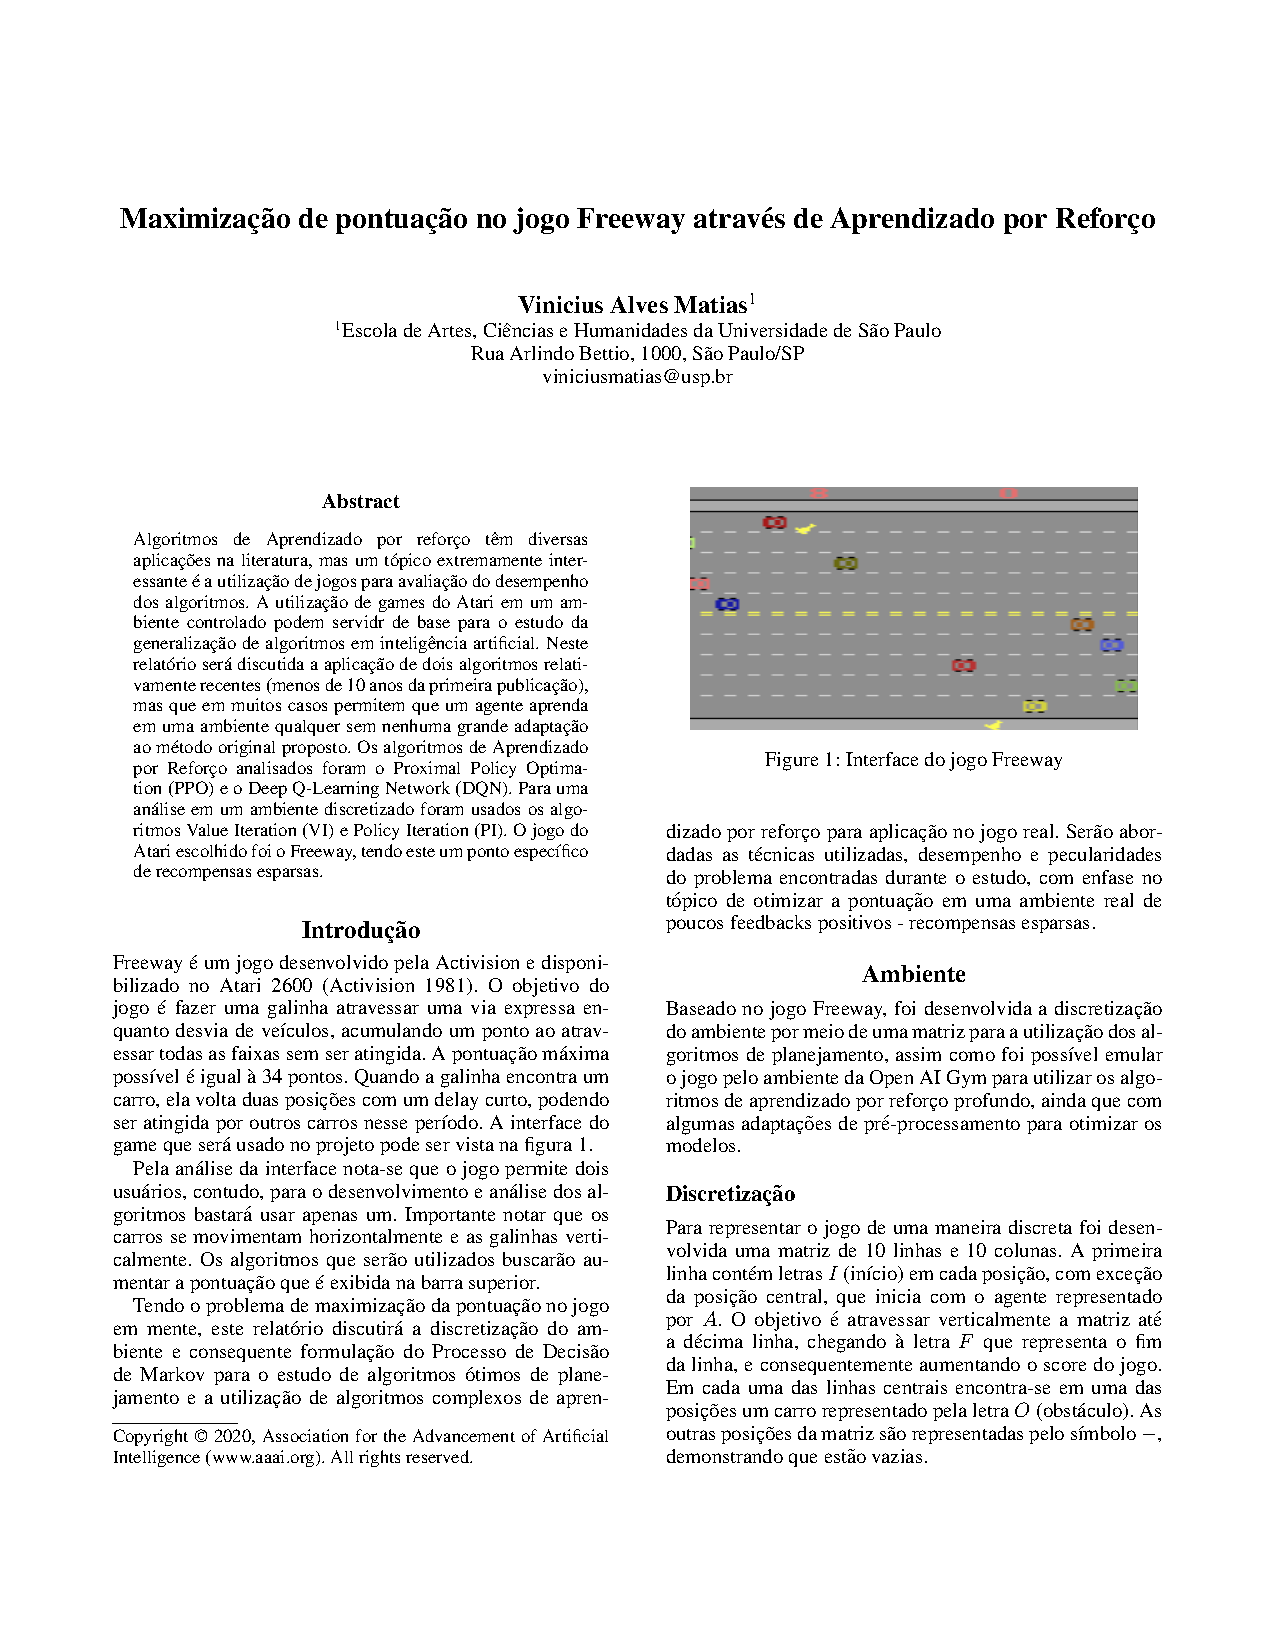
\includegraphics[width=0.9\columnwidth]{freeway}
\caption{Interface do jogo Freeway}
\label{freeway}
\end{figure}

Pela análise da interface nota-se que o jogo permite dois usuários, contudo, para o desenvolvimento e análise dos algoritmos bastará usar apenas um. Importante notar que os carros se movimentam horizontalmente e as galinhas verticalmente. Os algoritmos que serão utilizados buscarão aumentar a pontuação que é exibida na barra superior.

Tendo o problema de maximização da pontuação no jogo em mente, este relatório discutirá a discretização do ambiente e consequente formulação do Processo de Decisão de Markov para o estudo de algoritmos ótimos de planejamento e a utilização de algoritmos complexos de aprendizado por reforço para aplicação no jogo real. Serão abordadas as técnicas utilizadas, desempenho e pecularidades do problema encontradas durante o estudo, com enfase no tópico de otimizar a pontuação em uma ambiente real de poucos feedbacks positivos - recompensas esparsas.

\section{Ambiente}
Baseado no jogo Freeway, foi desenvolvida a discretização do ambiente por meio de uma matriz para a utilização dos algoritmos de planejamento, assim como foi possível emular o jogo pelo ambiente da Open AI Gym para utilizar os algoritmos de aprendizado por reforço profundo, ainda que com algumas adaptações de pré-processamento para otimizar os modelos.

\subsection{Discretização}
Para representar o jogo de uma maneira discreta foi desenvolvida uma matriz de 10 linhas e 10 colunas. A primeira linha contém letras $I$ (início) em cada posição, com exceção da posição central, que inicia com o agente representado por $A$. O objetivo é atravessar verticalmente a matriz até a décima linha, chegando à letra $F$ que representa o fim da linha, e consequentemente aumentando o score do jogo. Em cada uma das linhas centrais encontra-se em uma das posições um carro representado pela letra $O$ (obstáculo). As outras posições da matriz são representadas pelo símbolo $-$, demonstrando que estão vazias. 

Como o jogo tem um tempo limite de 136 segundos, o ambiente também terá um tempo delimitado especificado. Para este artigo seguimos que existirão 272 iterações, isto é, para milissegundo o agente poderá tomar uma ação, assim como os carros se moverão para a próxima posição válida na sua linha - da primeira à quarta linha vão para a direita, e da quinta à nona vão para a esquerda. Para o ambiente discreto não foi considerada uma velocidade específica para cada veículo, mas sim uma mesma para todos. A figura 2 exemplifica essa mudança do ambiente para uma próxima iteração.


\begin{figure}[h]
     \begin{subfigure}[h]{0.2\textwidth}
         \centering
         \includegraphics[width=\textwidth]{discreto_t1.png}
         \caption{Ambiente em $t$}
     \end{subfigure}
     \hfill
     \begin{subfigure}[h]{0.2\textwidth}
         \includegraphics[width=\textwidth]{discreto_t2.png}
         \caption{Ambiente em $t+1$}
     \end{subfigure}
        \caption{Matriz que representa o ambiente discreto em um momento $t$ (a) e $t+1$ (b)}
\end{figure}


\subsection{Pré-Processamento no Atari}
A velocidade para execução de algoritmos que têm relação à redes neurais muitas vezes é dependente da entrada recebida. Para otimizar os algoritmos PPO e DQN foi realizada um redimenstionamento nos frames enviados aos jogos. A dimensão de 210px (altura) por 160px (largura) passou para 84X84. Esse redimensionamento influenciou em mais agilidade para realizar os testes, visto que para o DQN (que será visto logo) sem nenhuma adaptação da imagem resultou uma rede neural com mais de 34 milhões de parâmetros possíveis, enquanto a adaptação resultou em cerca de 5 milhões de pesos possíveis. Para este momento do projeto não foram realizadas outras adaptações como na luminância, ajustes para escala de cinza ou junção de dimensões da imagem em um único canal, mencionados no artigo que propos o DQN.

\subsection{Recompensas esparsas}
Em planejamento, quando discretizamos o ambiente podemos facilmente determinar recompensas para incentivar o aprendizado de um agente. Isso implica que não teremos apenas recompensas positivas, mas também negativas facilmente detectáveis (chegar ao fim do trajeto é algo positivo e ser atingido por um obstáculo é negativo).

Em ambientes reais, contudo, a definição das recompensas deve estar atrelada ao que se tem disponível do ambiente, não sendo viável reallizar processamentos à mais para adicionar outros tipos de recompensas (como uma definição prévia de processamento para identificar veículos e então atualizá-los como recompensas negativas). Além de aumentar a complexidade do método, processamentos adicionais se afastariam da tentativa de um algoritmo de aprendizado por reforço aprender sem nenhuma interferência externa.

Isso leva à notar que nosso problema terá apenas uma recompensa bem definida à priori, que é chegar ao fim da via expressa (aumentar o score do jogo). Para adquirir essa recompensa, contudo, o agente deve passar por todos os obstáculos e então receber o feedback.

Isso não é tão incomum em jogos do Atari, tanto que os algoritmos PPO e DQN conseguem contornar esses problemas por intermédio da "janela" (buffer) que terão acesso para definir as melhores ações para um problema. O DQN em especial tem algo que salva muitos algoritmos do caso de recompensas esparsas: o fato de ser \textit{off-policy}, logo, ainda que busque a ação que otimize a recompensa em um estado, à uma probabilidade de desvirtuar dessa suposta melhor recompensa e, eventualmente, tornar o processo mais eficiente.

É importante notar que ainda que para o \textit{Freeway} as recompensas esparsas não sejam problemas muito grandes por haver um bom tratamento delas, em alguns problemas pode ser mais interessante buscar algoritmos que buscam explorar muito o ambiente em busca de informações que possam ser úteis posteriormente, isto é, algoritmos que "dirigidos à curiosidade" (Pathak et al. 2017) , que possivelmente teriam desempenho decente sob o jogo em questão 


\section{Planejamento Probabilístico}
O ambiente discretizado mencionado no item anterior é a base para a aplicação dos algoritmos de planejamento. Antes de iniciar esse estudo, note que a pontuação máxima para essa versão do jogo não é 34 pontos, pois temos 10 posições possíveis para o agente e 272 iterações, assim, a máxima pontuação possível será de $\lfloor \frac{272}{10}\rfloor = 27$ pontos. Com isto dito, podemos definir o MDP (\textit{Markov Decision Process}).

Um MDP é uma tupla ...


\subsection{Value Iteration}

\subsection{Policy iteration}

\section{Aprendizado por Reforço}

\subsection{Proximal Policy Optimization}

\subsection{Deep Q-Learning Network}
O algoritmo Deep Q-Learning Network foi proposto por uma equipe da DeepMind (Minth et al. 2013) em um artigo que ficou amplamente conhecido na área pela robustez do algoritmo. Com poucas alterações na estrutura descrita pelos autores o algoritmo pode ser adaptado à diferentes problemas e, muitas vezes, com desempenho sobre-humano quando falamos de jogos. Tal como o nome diz, esse algoritmo parte da definição do \textit{Q-Learning}:

$$
Q(s,a) = r(s,a) + \gamma max_a Q(s',a)
$$

Ainda que com certas semelhanças com o \textit{Value Iteration}, o \textit{Q-Learning} segue abordagens diferentes e entra no escopo de aprendizado por reforço, e não planejamento probabilístico. Na equação, $Q(s,a)$ é a soma da recompensa de se chegar em um estado $s$ com a ação $a$ somada ao próximo $Q(s',a)$ para uma ação $a$ que maximiza esse valor, descontada por um valor pré-definido $\gamma$. A recursão causada em $Q(s',a)$ é o que causa a convergência do \textit{Q-Learning}. A semelhança com o \textit{Value Iteration}, portanto, vem da questão da convergência, ou seja, da equação de \textit{Bellman}.

Uma coisa é convergência em ambientes discretos, em que a recorrência consiga ser definida, outra coisa totalmente diferente é a aplicação da recorrência em um ambiente que não temos conhecimento da quantidade de estados à priori, e nem temos ideia do fim do algoritmo. Para aplicar esse conceito em um ambiente real desconhecido que foi proposta a adição de redes neurais com uma maneira de armazenar Q valores anteriores nesse problema.

A rede neural servirá para estimar o \textit{Q-value} para um estado e ação (com pesos aleatórios no início, mas se adaptando conforme o treinamento), esse Q valor predito será batido com o valor real de se tomar essa ação e, assim, podemos computar a perda na rede neural como o quadrado da diferença entre o predito e a ação tomada. Uma abordagem fantástica que faz toda a diferença nesse processo é que nós armazenamos os últimos $n$ valores de Q para um um tupla estado-ação-estado predito, e durante a iteração da rede neural haverá uma probabilidade $1-\epsilon$ que normalmente é grande no início de tomarmos uma ação aleatória, mas que decresce no decorrer das iterações, e isso implica em escolhermos uma ação que maximize o \textit{Q-value} dentro da rede neural para um par estado-ação muitas vezes, mas com um probabilidade baixa de procurarmos outra ação.

2 anos depois a DeepMind publicou outro artigo trazendo uma abordagem possível para treinamento de jogos no Atari, consistindo da utilização de redes convolucionais para tratar a entrada (e processá-la na rede) e por fim passá-la para uma camada profunda que terá como saída as ações possíveis de serem tomadas no jogo. Para o problema de maximização no \textit{Freeway}, fizemos algumas adaptações à fim de criar um rede com a seguinte configuração: 

\begin{itemize}
	\item Uma entrada de frames 84X84X3 (3 canais);
	\item Uma camada oculta de 32 filtros 8X8 com stride 4 e função de ativação ReLU (convolutional);
	\item Uma camada oculta de 64 filtros 4X4 com stride 2 e função de ativação ReLU (convolutional);
	\item Uma camada oculta de 64 filtros 3X3 com stride 1 e função de ativação ReLU (convolutional);
	\item Uma camada \textit{Flatten} para intermediar as camadas convolucionais e densas
	\item Uma camada oculta de 512 perceptrons e função de ativação ReLU (densa)
	\item Uma camada oculta de 256 perceptrons e função de ativação ReLU (densa)
	\item Uma camada oculta de 3 perceptrons (quantidade de ações) e função de ativação ReLU (densa)
\end{itemize}

Os resultados podem ser vistos na figura à seguir.

\begin{figure}[h]
     \begin{subfigure}[h]{0.2\textwidth}
         \centering
         \includegraphics[width=\textwidth]{dqn_100k}
         \caption{100 mil passos}
     \end{subfigure}
     \hfill
     \begin{subfigure}[h]{0.2\textwidth}
         \includegraphics[width=\textwidth]{1M_dqn_passos}
         \caption{1 milhão de passos}
     \end{subfigure}
        \caption{Curva de aumento na pontuação para 100 mil passos (a) e 1 milhão de passos (b)}
\end{figure}

\section{Desempenho dos algoritmos}



\section{Conclusão}

\section{Referências}
\end{document}
